\setAuthor{Moorits Mihkel Muru}
\setRound{piirkonnavoor}
\setYear{2024}
\setNumber{G 2}
\setDifficulty{2}
\setTopic{TODO}

\prob{Hajumine}
Juhanil on valgusallikas, mis tekitab paralleelset silindrikujulist valgusvihku, ning väike fotodetektorist tajur, mis mõõdab valguse intensiivsust. Esimeses katses mõõdab Juhan valgusallika intensiivsust, asetades tajuri täielikult valgusallika valgusvihku (ilma kumerpeeglita). Teises katses (vt joonis) suunab Juhan valgusvihu kumerpeeglile, mille kumerusraadius on $R=\SI{30}{\centi\m}$, nii et valgusvihk asub optilisel peateljel ja on sellega paralleelne. Seejärel mõõdab Juhan hajunud valguse intensiivsust, asetades tajuri täielikult peegeldunud valgusvihku (aga valgusallika enda valgusvihust kõrvale) peegli pinnast $L=\SI{60}{\centi\m}$ kaugusele. Mitu korda on tajuri näit esimeses katses suurem kui teises katses? Võib eeldada, et valgusallika valgusvihu laius on palju väiksem peegli kumerusraadiusest.

\begin{figure}[h]
    \centering
    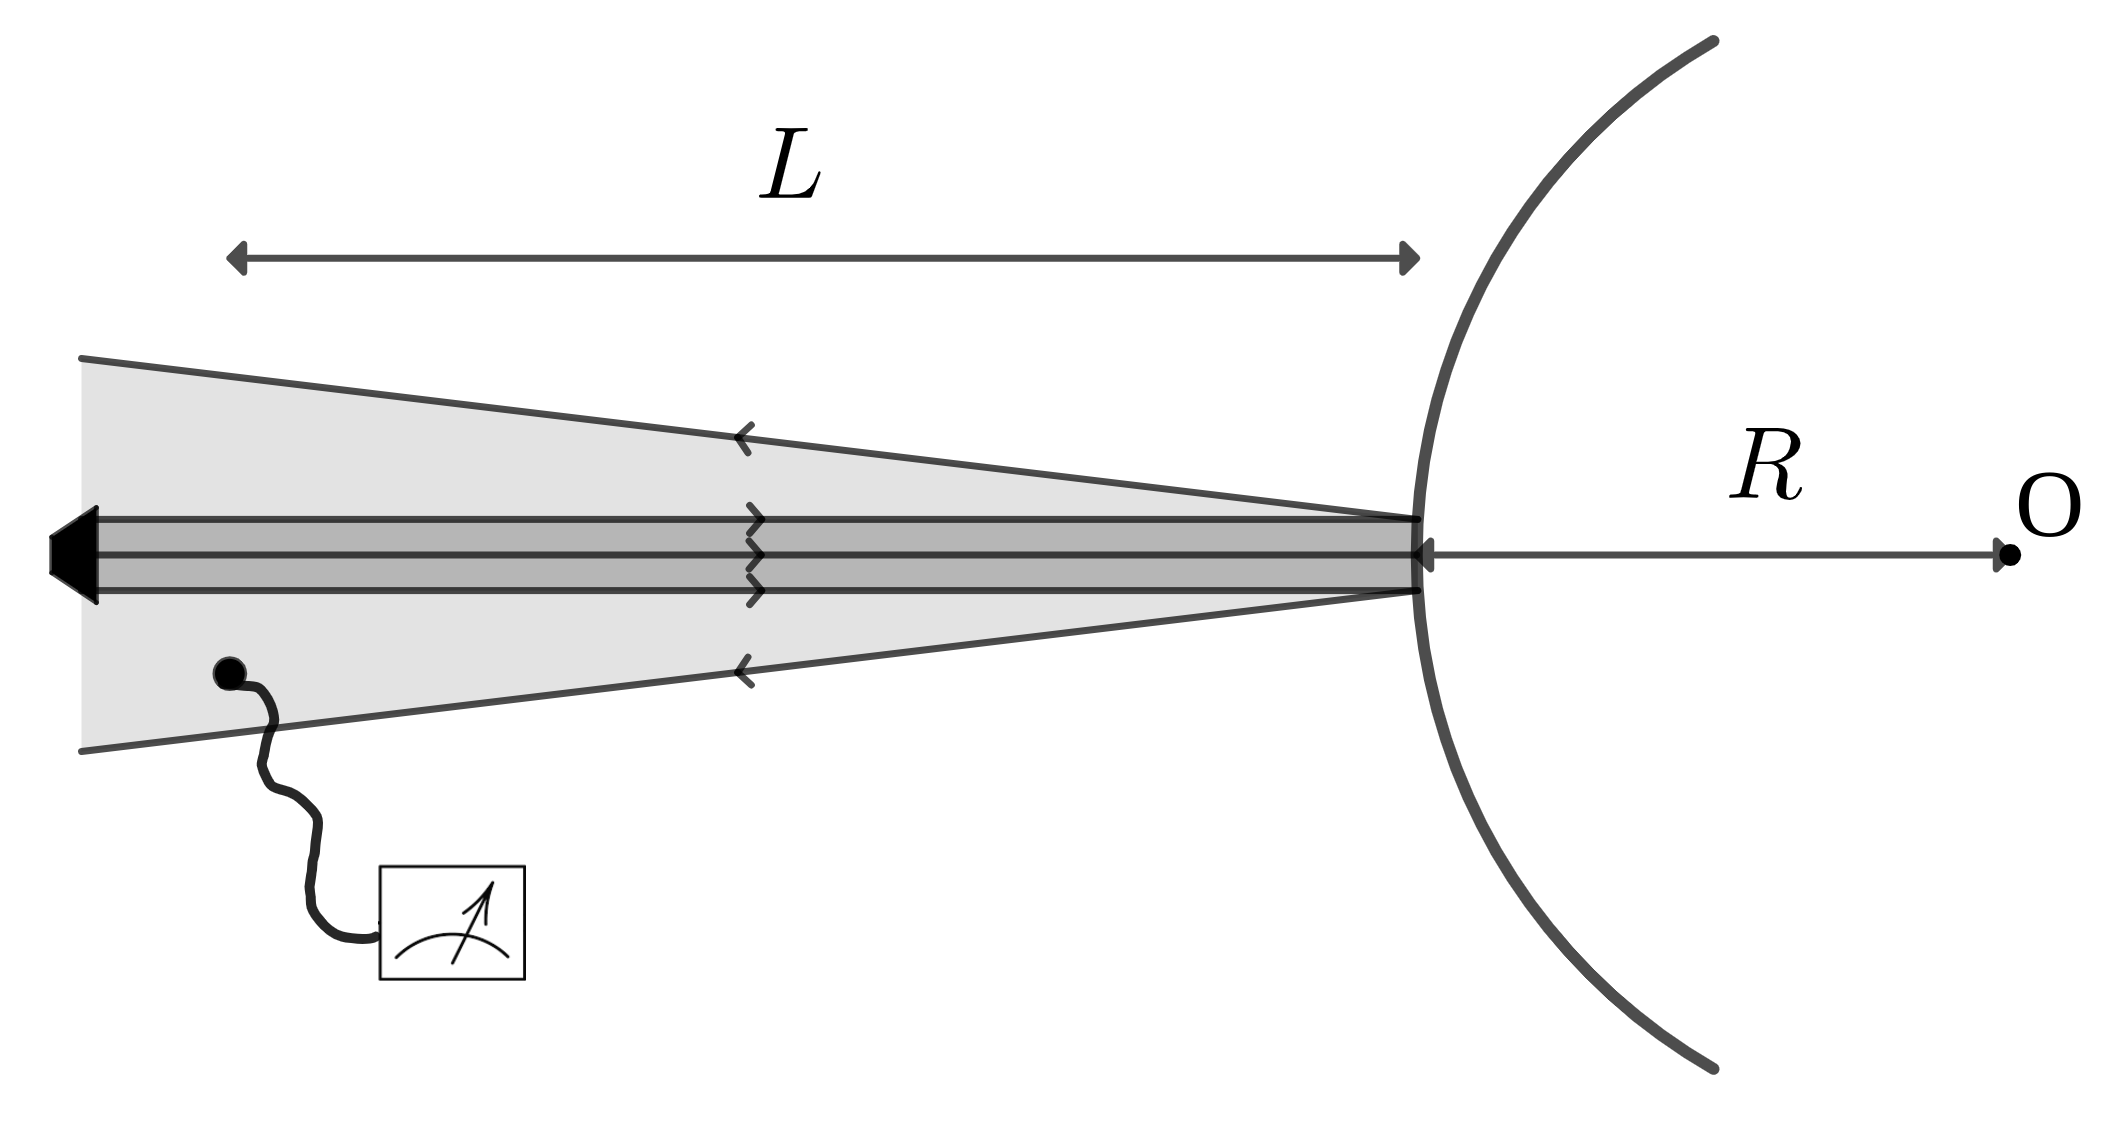
\includegraphics[width=0.6\linewidth]{2024-v2g-02-yl.png}
\end{figure}




\hint

\solu
Tajur mõõdab valgustihedust ehk valgustatust, seega mida suurema ala peale valgusallikast pärinev valgus hajub, seda väiksem on tajuri näit. Olgu valgusallika võimsus $P$ ja valgusallikast tuleva valgusvihu pindala $S_1$, siis esimeses katses mõõdetud tajuri näitu kirjeldab suurus $E_1 = P/S_1 = P/\pi r_1^2$, kui eeldada, et valgusvihu pindala on ringikujuline ja raadiusega $r_1$. Teises katses kirjeldab tajuri väärtust suurus $E_2 = P/S_2 = P/\pi r_2^2$, kus $r_2$ sõltub sellest, kui kaugel tajur peeglist on. Raadiuse $r_2$ saab avaldada läbi raadiuse $r_1$ kasutades teadmist, et kumerpeeglile lastud paralleelne kiirtekimp koondub fookuses, mis asub kumerpeegli pinnast kaugusel $R/2$. Tekivad sarnased kolmnurgad, millest esimese kõrgus on $R/2$ ja alus $2r_1$ ning teise kõrgus on $R/2 + L$ ning alus $2r_2$. Seega saame
$$ \frac{R/2}{2r_1} = \frac{R/2 + L}{2r_2} \Rightarrow r_2 = \frac{R/2 + L}{R/2} r_1$$
ja tajuri näitude suhe on
$$ \frac{E_1}{E_2} = \frac{P/S_1}{P/S_2} = \frac{S_2}{S_1} = \frac{r_2^2}{r_1^2} = \left(\frac{R/2 + L}{R/2}\right)^2 = \left(\frac{\SI{15}{\centi\meter} + \SI{60}{\centi\meter}}{\SI{15}{\centi\meter}}\right)^2 = 25 \ .$$

\begin{figure}[h]
    \centering
    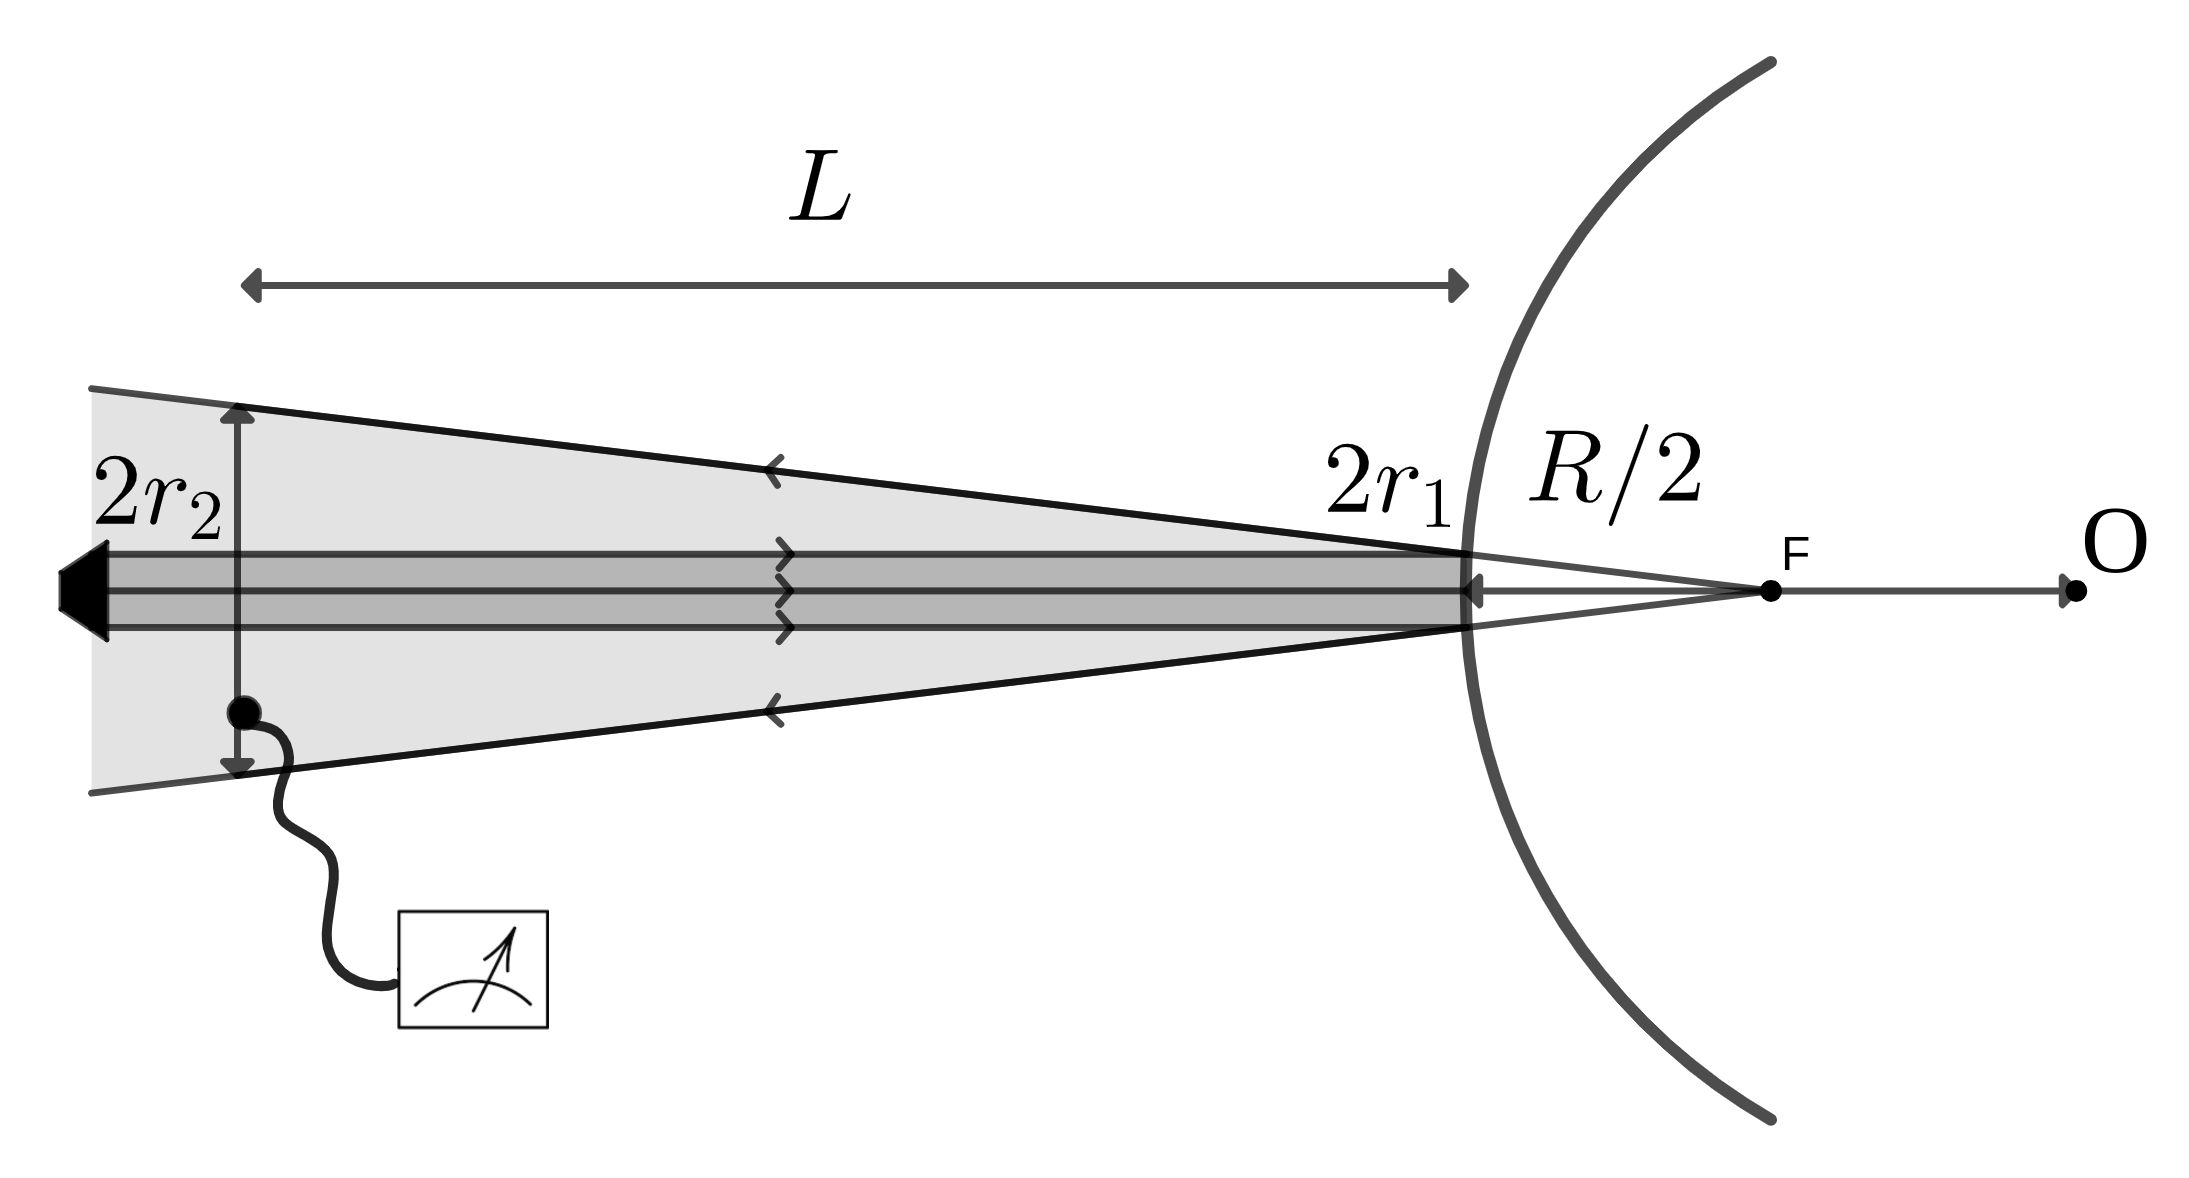
\includegraphics[width=0.6\linewidth]{2024-v2g-02-sol.png}
\end{figure}
\probend